% *** Authors should verify (and, if needed, correct) their LaTeX system  ***
% *** with the testflow diagnostic prior to trusting their LaTeX platform ***
% *** with production work. IEEE's font choices and paper sizes can       ***
% *** trigger bugs that do not appear when using other class files.       ***                          ***
% The testflow support page is at:
% http://www.michaelshell.org/tex/testflow/



\documentclass[conference,compsoc]{IEEEtran}
% Some/most Computer Society conferences require the compsoc mode option,
% but others may want the standard conference format.
%
% If IEEEtran.cls has not been installed into the LaTeX system files,
% manually specify the path to it like:
% \documentclass[conference,compsoc]{../sty/IEEEtran}
\usepackage{hyperref}
\usepackage{graphicx}



% Some very useful LaTeX packages include:
% (uncomment the ones you want to load)


% *** MISC UTILITY PACKAGES ***
%
%\usepackage{ifpdf}
% Heiko Oberdiek's ifpdf.sty is very useful if you need conditional
% compilation based on whether the output is pdf or dvi.
% usage:
% \ifpdf
%   % pdf code
% \else
%   % dvi code
% \fi
% The latest version of ifpdf.sty can be obtained from:
% http://www.ctan.org/tex-archive/macros/latex/contrib/oberdiek/
% Also, note that IEEEtran.cls V1.7 and later provides a builtin
% \ifCLASSINFOpdf conditional that works the same way.
% When switching from latex to pdflatex and vice-versa, the compiler may
% have to be run twice to clear warning/error messages.






% *** CITATION PACKAGES ***
%
\ifCLASSOPTIONcompsoc
  % IEEE Computer Society needs nocompress option
  % requires cite.sty v4.0 or later (November 2003)
  \usepackage[nocompress]{cite}
\else
  % normal IEEE
  \usepackage{cite}
\fi
% cite.sty was written by Donald Arseneau
% V1.6 and later of IEEEtran pre-defines the format of the cite.sty package
% \cite{} output to follow that of IEEE. Loading the cite package will
% result in citation numbers being automatically sorted and properly
% "compressed/ranged". e.g., [1], [9], [2], [7], [5], [6] without using
% cite.sty will become [1], [2], [5]--[7], [9] using cite.sty. cite.sty's
% \cite will automatically add leading space, if needed. Use cite.sty's
% noadjust option (cite.sty V3.8 and later) if you want to turn this off
% such as if a citation ever needs to be enclosed in parenthesis.
% cite.sty is already installed on most LaTeX systems. Be sure and use
% version 5.0 (2009-03-20) and later if using hyperref.sty.
% The latest version can be obtained at:
% http://www.ctan.org/tex-archive/macros/latex/contrib/cite/
% The documentation is contained in the cite.sty file itself.
%
% Note that some packages require special options to format as the Computer
% Society requires. In particular, Computer Society  papers do not use
% compressed citation ranges as is done in typical IEEE papers
% (e.g., [1]-[4]). Instead, they list every citation separately in order
% (e.g., [1], [2], [3], [4]). To get the latter we need to load the cite
% package with the nocompress option which is supported by cite.sty v4.0
% and later.





% *** GRAPHICS RELATED PACKAGES ***
%
\ifCLASSINFOpdf
  % \usepackage[pdftex]{graphicx}
  % declare the path(s) where your graphic files are
  % \graphicspath{{../pdf/}{../jpeg/}}
  % and their extensions so you won't have to specify these with
  % every instance of \includegraphics
  % \DeclareGraphicsExtensions{.pdf,.jpeg,.png}
\else
  % or other class option (dvipsone, dvipdf, if not using dvips). graphicx
  % will default to the driver specified in the system graphics.cfg if no
  % driver is specified.
  % \usepackage[dvips]{graphicx}
  % declare the path(s) where your graphic files are
  % \graphicspath{{../eps/}}
  % and their extensions so you won't have to specify these with
  % every instance of \includegraphics
  % \DeclareGraphicsExtensions{.eps}
\fi
% graphicx was written by David Carlisle and Sebastian Rahtz. It is
% required if you want graphics, photos, etc. graphicx.sty is already
% installed on most LaTeX systems. The latest version and documentation
% can be obtained at: 
% http://www.ctan.org/tex-archive/macros/latex/required/graphics/
% Another good source of documentation is "Using Imported Graphics in
% LaTeX2e" by Keith Reckdahl which can be found at:
% http://www.ctan.org/tex-archive/info/epslatex/
%
% latex, and pdflatex in dvi mode, support graphics in encapsulated
% postscript (.eps) format. pdflatex in pdf mode supports graphics
% in .pdf, .jpeg, .png and .mps (metapost) formats. Users should ensure
% that all non-photo figures use a vector format (.eps, .pdf, .mps) and
% not a bitmapped formats (.jpeg, .png). IEEE frowns on bitmapped formats
% which can result in "jaggedy"/blurry rendering of lines and letters as
% well as large increases in file sizes.
%
% You can find documentation about the pdfTeX application at:
% http://www.tug.org/applications/pdftex





% *** MATH PACKAGES ***
%
%\usepackage[cmex10]{amsmath}
% A popular package from the American Mathematical Society that provides
% many useful and powerful commands for dealing with mathematics. If using
% it, be sure to load this package with the cmex10 option to ensure that
% only type 1 fonts will utilized at all point sizes. Without this option,
% it is possible that some math symbols, particularly those within
% footnotes, will be rendered in bitmap form which will result in a
% document that can not be IEEE Xplore compliant!
%
% Also, note that the amsmath package sets \interdisplaylinepenalty to 10000
% thus preventing page breaks from occurring within multiline equations. Use:
%\interdisplaylinepenalty=2500
% after loading amsmath to restore such page breaks as IEEEtran.cls normally
% does. amsmath.sty is already installed on most LaTeX systems. The latest
% version and documentation can be obtained at:
% http://www.ctan.org/tex-archive/macros/latex/required/amslatex/math/





% *** SPECIALIZED LIST PACKAGES ***
%
%\usepackage{algorithmic}
% algorithmic.sty was written by Peter Williams and Rogerio Brito.
% This package provides an algorithmic environment fo describing algorithms.
% You can use the algorithmic environment in-text or within a figure
% environment to provide for a floating algorithm. Do NOT use the algorithm
% floating environment provided by algorithm.sty (by the same authors) or
% algorithm2e.sty (by Christophe Fiorio) as IEEE does not use dedicated
% algorithm float types and packages that provide these will not provide
% correct IEEE style captions. The latest version and documentation of
% algorithmic.sty can be obtained at:
% http://www.ctan.org/tex-archive/macros/latex/contrib/algorithms/
% There is also a support site at:
% http://algorithms.berlios.de/index.html
% Also of interest may be the (relatively newer and more customizable)
% algorithmicx.sty package by Szasz Janos:
% http://www.ctan.org/tex-archive/macros/latex/contrib/algorithmicx/




% *** ALIGNMENT PACKAGES ***
%
%\usepackage{array}
% Frank Mittelbach's and David Carlisle's array.sty patches and improves
% the standard LaTeX2e array and tabular environments to provide better
% appearance and additional user controls. As the default LaTeX2e table
% generation code is lacking to the point of almost being broken with
% respect to the quality of the end results, all users are strongly
% advised to use an enhanced (at the very least that provided by array.sty)
% set of table tools. array.sty is already installed on most systems. The
% latest version and documentation can be obtained at:
% http://www.ctan.org/tex-archive/macros/latex/required/tools/


% IEEEtran contains the IEEEeqnarray family of commands that can be used to
% generate multiline equations as well as matrices, tables, etc., of high
% quality.




% *** SUBFIGURE PACKAGES ***
%\ifCLASSOPTIONcompsoc
%  \usepackage[caption=false,font=footnotesize,labelfont=sf,textfont=sf]{subfig}
%\else
%  \usepackage[caption=false,font=footnotesize]{subfig}
%\fi
% subfig.sty, written by Steven Douglas Cochran, is the modern replacement
% for subfigure.sty, the latter of which is no longer maintained and is
% incompatible with some LaTeX packages including fixltx2e. However,
% subfig.sty requires and automatically loads Axel Sommerfeldt's caption.sty
% which will override IEEEtran.cls' handling of captions and this will result
% in non-IEEE style figure/table captions. To prevent this problem, be sure
% and invoke subfig.sty's "caption=false" package option (available since
% subfig.sty version 1.3, 2005/06/28) as this is will preserve IEEEtran.cls
% handling of captions.
% Note that the Computer Society format requires a sans serif font rather
% than the serif font used in traditional IEEE formatting and thus the need
% to invoke different subfig.sty package options depending on whether
% compsoc mode has been enabled.
%
% The latest version and documentation of subfig.sty can be obtained at:
% http://www.ctan.org/tex-archive/macros/latex/contrib/subfig/




% *** FLOAT PACKAGES ***
%
%\usepackage{fixltx2e}
% fixltx2e, the successor to the earlier fix2col.sty, was written by
% Frank Mittelbach and David Carlisle. This package corrects a few problems
% in the LaTeX2e kernel, the most notable of which is that in current
% LaTeX2e releases, the ordering of single and double column floats is not
% guaranteed to be preserved. Thus, an unpatched LaTeX2e can allow a
% single column figure to be placed prior to an earlier double column
% figure. The latest version and documentation can be found at:
% http://www.ctan.org/tex-archive/macros/latex/base/


%\usepackage{stfloats}
% stfloats.sty was written by Sigitas Tolusis. This package gives LaTeX2e
% the ability to do double column floats at the bottom of the page as well
% as the top. (e.g., "\begin{figure*}[!b]" is not normally possible in
% LaTeX2e). It also provides a command:
%\fnbelowfloat
% to enable the placement of footnotes below bottom floats (the standard
% LaTeX2e kernel puts them above bottom floats). This is an invasive package
% which rewrites many portions of the LaTeX2e float routines. It may not work
% with other packages that modify the LaTeX2e float routines. The latest
% version and documentation can be obtained at:
% http://www.ctan.org/tex-archive/macros/latex/contrib/sttools/
% Do not use the stfloats baselinefloat ability as IEEE does not allow
% \baselineskip to stretch. Authors submitting work to the IEEE should note
% that IEEE rarely uses double column equations and that authors should try
% to avoid such use. Do not be tempted to use the cuted.sty or midfloat.sty
% packages (also by Sigitas Tolusis) as IEEE does not format its papers in
% such ways.
% Do not attempt to use stfloats with fixltx2e as they are incompatible.
% Instead, use Morten Hogholm'a dblfloatfix which combines the features
% of both fixltx2e and stfloats:
%
% \usepackage{dblfloatfix}
% The latest version can be found at:
% http://www.ctan.org/tex-archive/macros/latex/contrib/dblfloatfix/




% *** PDF, URL AND HYPERLINK PACKAGES ***
%
%\usepackage{url}
% url.sty was written by Donald Arseneau. It provides better support for
% handling and breaking URLs. url.sty is already installed on most LaTeX
% systems. The latest version and documentation can be obtained at:
% http://www.ctan.org/tex-archive/macros/latex/contrib/url/
% Basically, \url{my_url_here}.




% *** Do not adjust lengths that control margins, column widths, etc. ***
% *** Do not use packages that alter fonts (such as pslatex).         ***
% There should be no need to do such things with IEEEtran.cls V1.6 and later.
% (Unless specifically asked to do so by the journal or conference you plan
% to submit to, of course. )


% correct bad hyphenation here
\hyphenation{op-tical net-works semi-conduc-tor}


\begin{document}

%
% paper title
% Titles are generally capitalized except for words such as a, an, and, as,
% at, but, by, for, in, nor, of, on, or, the, to and up, which are usually
% not capitalized unless they are the first or last word of the title.
% Linebreaks \\ can be used within to get better formatting as desired.
% Do not put math or special symbols in the title.
\title{MAIG Individual Assignment}


% author names and affiliations
% use a multiple column layout for up to three different
% affiliations
\author{
\IEEEauthorblockN{Mikkel Stolborg}
\IEEEauthorblockA{Games and Technology\\
IT-University of Copenhagen\\
Copenhagen, Denmark\\
Email: msto@itu.dk}
% Template for adding other people
%\and
%\IEEEauthorblockN{Homer Simpson}
%\IEEEauthorblockA{Twentieth Century Fox\\
%Springfield, USA\\
%Email: homer@thesimpsons.com}
%\and
%\IEEEauthorblockN{James Kirk\\ and Montgomery Scott}
%\IEEEauthorblockA{Starfleet Academy\\
%San Francisco, California 96678-2391\\
%Telephone: (800) 555--1212\\
%Fax: (888) 555--1212}
}

% conference papers do not typically use \thanks and this command
% is locked out in conference mode. If really needed, such as for
% the acknowledgment of grants, issue a \IEEEoverridecommandlockouts
% after \documentclass

% for over three affiliations, or if they all won't fit within the width
% of the page (and note that there is less available width in this regard for
% compsoc conferences compared to traditional conferences), use this
% alternative format:
% 
%\author{\IEEEauthorblockN{Michael Shell\IEEEauthorrefmark{1},
%Homer Simpson\IEEEauthorrefmark{2},
%James Kirk\IEEEauthorrefmark{3}, 
%Montgomery Scott\IEEEauthorrefmark{3} and
%Eldon Tyrell\IEEEauthorrefmark{4}}
%\IEEEauthorblockA{\IEEEauthorrefmark{1}School of Electrical and Computer Engineering\\
%Georgia Institute of Technology,
%Atlanta, Georgia 30332--0250\\ Email: see http://www.michaelshell.org/contact.html}
%\IEEEauthorblockA{\IEEEauthorrefmark{2}Twentieth Century Fox, Springfield, USA\\
%Email: homer@thesimpsons.com}
%\IEEEauthorblockA{\IEEEauthorrefmark{3}Starfleet Academy, San Francisco, California 96678-2391\\
%Telephone: (800) 555--1212, Fax: (888) 555--1212}
%\IEEEauthorblockA{\IEEEauthorrefmark{4}Tyrell Inc., 123 Replicant Street, Los Angeles, California 90210--4321}}




% use for special paper notices
%\IEEEspecialpapernotice{(Invited Paper)}




% make the title area
\maketitle

% As a general rule, do not put math, special symbols or citations
% in the abstract
\begin{abstract}
The abstract goes here.
\end{abstract}

% no keywords




% For peer review papers, you can put extra information on the cover
% page as needed:
% \ifCLASSOPTIONpeerreview
% \begin{center} \bfseries EDICS Category: 3-BBND \end{center}
% \fi
%
% For peerreview papers, this IEEEtran command inserts a page break and
% creates the second title. It will be ignored for other modes.
\IEEEpeerreviewmaketitle



\section{Introduction}
% no \IEEEPARstart
This report contains the dissertation of 3 methods used to create an AI for the \textit{Ms. PacMan Vs Ghosts} framework.
The 3 methods in question are an AI using a \textit{Behaviour Tree}, one using a \textit{Monte Carlo Tree Search} algorithm, and one using a \textit{State Machine} optimized by a \textit{Genetic Algorithm}.

For each of the methods and their algorithms I will detail the approach to the problem, which considerations were made before tackling the task at hand, the parameters of the algorithm, the parameters the final algorithm uses for the AI, and the performance measure of the algorithm, the scores the AI achieves over a number of games, totalling the average value, the minimum, and the maximum score.

Finally I will compare the performance of each of the AI's to the performance of the AI' included in the \textit{Ms. PacMan Vs Ghosts} framework.

\section{Behaviour Tree}
In this section I go over the approach for the behaviour tree based AI, the parameters the AI uses, and how well it performs on average.
\subsection{Description of Approach}
\begin{figure}[h]
	\graphicspath{{figures/}}
	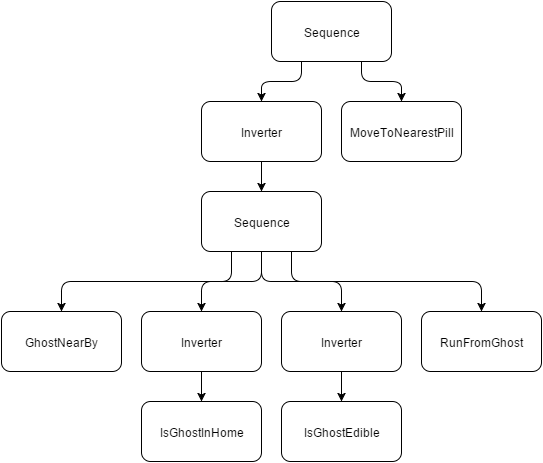
\includegraphics[scale=0.5]{ModernAIBehaviourTree.png}
	\caption{Behaviour tree for final AI. The top sequence is the entry point. The left branch returns true if there are no ghost nearby.}
	\label{fig:behavTree}
\end{figure}
A behaviour tree is a tree structure that you traverse using its own logic to find a action to take. The nodes in the ends of the tree are called leafs, and they decide which action the AI takes. 
The structure of the tree contains several types of nodes which helps run the correct leafs and executing the correct action. 
Each of the leafs returns one of 3 values, running, failure, or success. The leaf executes its code and depending of whether it failed, no ghost nearby, succeed, ghost are nearby, or running, when it is still processing its action, moving towards nearest pill.
Each of the other nodes are controlled by the responses from the leaves. The categories for the nodes, other than leaf, are \textit{Decorator} and \textit{Composite}.

The composite node is capable of having several child nodes. A good example of a composite node is the sequence node. The sequence node runs through all of its children, starting from the first added, until it reaches the end or when a child fails. On failure of a child the sequence returns failure, it returns running if the current child it is investigating returns running, or success if all its children returns success. This type of sequence could be described as an and-loop. There exist the opposite loop, which could be described as an or-loop.

The decorator node is capable of having only a single child. A good example of a decorator node is the inverter used in our algorithm. The inverter takes the input from its child and simply inverts it, returning success if the child failed or failure if the child succeed.

The strength of a behaviour tree is its modulation. Each of the leaf can be used independently of each other, and adding steps and conditions before an action, is merely the result of adding new leafs in between the existing ones.

The first approach was to create a simple AI, which simply tried to go to the nearest pill and eat it. This was achieved just by having a leaf in the tree which set the move of the tree result to send PacMan to the nearest available pill. This leaf was called MoveToNearLeaf. 

Now this AI obviously did not perform that well, as it completely ignored the ghost. In order to improve this I changed the root of the tree to a sequence and added logic to check for ghosts. The branch for getting the pills remained unchanged and the new branch for the ghost detection was added. The ghost detection were comprised of a sequence which would first check if there were ghost nearby, then if it were true, it would run from the ghost.

This improved upon the AI, however, it still did not behave as expected. It kept running from ghost, even edible ones and the ones in the lair. 
In order to fix this two new leafs were created, one to check if the ghost were edible and one to check if they were within their lair.
The final tree can be seen in figure \ref{fig:behavTree}.

\subsection{Algorithm Parameters}
The only parameter the algorithm uses is the distance of how close the ghost is allowed to be, before the AI will run from it. 
The parameter were set from the same as what the starter AI used, which proved to be efficient enough for the AI to execute its logic. 
\subsection{Performance measure of the algorithm}
In order to test the performance of the AI algorithm, we run 10 simulated games and collect the data of the experiment. The results can be seen in table \ref{tab:behavPer}.
\begin{table}[h]
\begin{center}
\begin{tabular}{|c|c|}
\hline
Max Score & 5560\\
\hline
Min Score & 2010\\
\hline
Average Score & 2914.0\\
\hline
\end{tabular}
\end{center}
\caption{Performance of the behaviour tree. The table includes the min score, max score, and the average score.}
\label{tab:behavPer}
\end{table}

The performance of the AI varies a lot, and it does not perform that well. This can be attributed to the fact that the AI does not chase the ghost, which are a source for greater points than simply succeeding in gathering pills. 

In order to improve the score of the AI, a branch could be included in the behaviour tree which is responsible for hunting and eating ghost when applicable. This could even be done using some of the leaves already in the current tree. 
\section{Monte Carlo Tree Search}
In this section I go over the approach for the \textit{Monte Carlo Tree Search} based AI, the parameters the AI uses, and how well it performs on average.
\subsection{Description of Approach}
A Monte Carlo Tree Search algorithm creates a partial tree of the entire game and from the limited knowledge choosing the best action to perform at the current state of the game. 

The way it achieves this is as follows. First it takes the current state as the root node of the search tree. Then while the tree still has time to compute, use the \textit{TreePolicy} on the node find the next node to investigate. 

The TreePolicy expands all the possible moves from the current state of the game. Then it return the \textit{BestChild} of the expanded nodes using an \textit{Upper Confidence Bound for Trees} (UCT) algorithm to estimate which child is the best.

The algorithm then uses \textit{DefaultPolicy} to determine a value for the chosen game node. This keeps making random choices till the game reaches an end state or some other predefined condition is achieved. Then it returns the reward of the end state to the main function. The reward is determined by what the developer wishes the AI to achieve. In this case the score achieved were used as reward.

Finally the algorithm walks back up the tree and adds the reward from the DefaultPolicy to each of the parent nodes in the \textit{Backup} function.

The result of the algorithm is the BestChild of the root node based on the total reward propagated back up through the tree.

The way the algorithm were implemented were to set the reward from the DefaultPolicy to be the reward. This way we tried to optimize the path taking into account the greater the score the more pills and the more ghost would be eaten.
\subsection{Algorithm Parameters}
The algorithm's only parameter is the parameter for how much the algorithm favours exploration. The parameter were determined solely through trial an error, and was settled on the value of 10. 
\subsection{Performance measure of the algorithm}
In order to test the performance of the AI algorithm, we run 10 simulated games and collect the data of the experiment. The results can be seen in table \ref{tab:MCTSPer}.
\begin{table}[h]
\begin{center}
\begin{tabular}{|c|c|}
\hline
Max Score & 780\\
\hline
Min Score & 300\\
\hline
Average Score & 543.0\\
\hline
\end{tabular}
\end{center}
\caption{Performance of the MCTS AI. The table includes the min score, max score, and the average score.}
\label{tab:MCTSPer}
\end{table}
The algorithm does not perform very well. This can be attributed to the fact that the AI is not punished significantly for being eaten by ghost. What is not shown in the table is the time it takes for the AI to die. It is actually able to avoid ghost because of the score wont increase if it is eaten. But the simple requirements does mean that it often just walks around in circles or back and forth. 
You could improve the AI significantly by punishing the reward if pacman gets eaten or if it keeps walking back and forth.
\section{State Machine and Genetic Algorithm}
In this section I go over the approach for the State machine based AI which were optimized using a Genetic Algorithm. I look in to the final parameters and how they were attained and I test how well it performs on average.
\subsection{Description of Approach}
First part of the AI were to create a suitable state machine. The machine had to take parameters which could be manipulated through a genetic algorithm. Second part were to create a genetic algorithm and have it optimize the variables available.

State machine works by having several states of actions, which jumps to the other states depending on different criteria. A special quirk with this state machine is that it first checks whether it should change state, rather than executing its own state first. 

The chosen states were as follows, an overview can be seen in figure \ref{fig:StateMach}. RunFromGhost is, as the name implies, the state of running from the ghosts. If the distance to a power pill is within its limits it will try to run towards it, by changing state to MoveToNearestPowerPill. If it simply evades the ghost it will revert to MoveToNearestPill.

MoveToNearestPowerPill moves towards the nearest power pill. The state will revert back to RunFromGhost if a ghost comes to close to it, as in a new ghost appear to kill it. It can go to the EatGhost state when it achieves eating a power pill. It defaults back to MoveToNearestPill if there are no ghost close.

EatGhost tries to eat any nearby ghost, in effect chasing after them. The state will revert back to MoveToNearestPill, if there is no edible ghost nearby.
\begin{figure}[h]
	\graphicspath{{figures/}}
	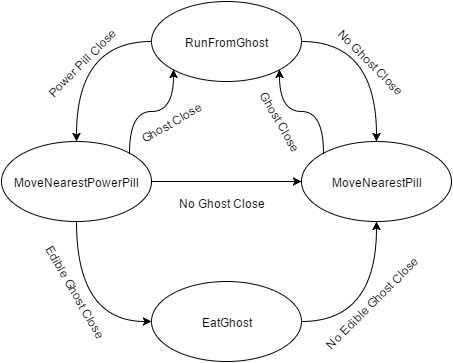
\includegraphics[scale=0.5]{StateMachineDiagram.png}
	\caption{State machine diagram. The 4 different state of the machine and the conditions for the changes between them.}
	\label{fig:StateMach}
\end{figure}

After the state machine were in place, a genetic algorithm were to optimize its parameters.

A genetic algorithm takes a population of genes and creates a new population based thereupon. The mechanisms for creating the new population varies, but mostly is done through reproduction and/or mutation. In this case we use both of the concepts as the simplicity of the genes, but the importance of the variables required both.
The genes map to what is called a phenotype, which is what the real representation of the population, in our case the state machine. 
Each gene has an associated fitness value, the value which determines how well the gene does in its environment. In our case the score which the state machine achieved is used as the fitness. 
The population, a number of genes, is usually kept constant. This is done through discarding members after each cycle. This will be explained below.

Reproduction is when you take members of your population and use them to create new individuals. The number of individuals created and the method through which it is done usually varies from each algorithm. The members used are usually the fittest members of the current population, but for diversity one could also include some of the worst members. 

The way members were reproduced in this case were through taking, at random, a piece of the chromosome from a parent and setting to be the child value. The reproduction method in this case also only creates one new member with two parents as input. 

Mutation is when you take an individual in your population and make a small random change in it. In this case a gene's chromosome, chosen at random, is varied by either increasing it by 1 or decreasing it by 1. 

In order to keep a constant population, usually only the fittest members survive each iteration of the algorithm. A gene can be discarded usually either due to age or to low fitness. In this case half of the population is discarded based solely on their fitness value.

The cycle of creating a new population is done until either a threshold in fitness is reached or a number of generations has occurred.

The algorithm were set to use the parameters of the state machine as its chromosome within its genes. 

\subsection{Algorithm Parameters}
The genetic algorithm uses the parameters of the state machine as its chromosomes for gene representation.
The parameters in question are those which decides when the states should be changed and are as follows:
\begin{itemize}
\item[]  \textbf{DistFromNonEdible}. The distance of non edible ghost. Used to determine when to run.
\item[] \textbf{DistToPowerPill}. The distance to the power pill. Used to determine if power pills are close enough.
\item[] \textbf{DistToEdible}. The distance to edible ghost. Used to determine if it is worth chasing ghost.
\end{itemize}

The parameters are randomized to a start value between 1 and 100. This max limit is chosen based on the general idea of the game size, and the minimum due to the requirement for it to be a positive non-negative number.
Furthermore the value is limited within the iteration of the algorithm to never go below 1.

The final value of the parameters of the algorithm and the start values can be seen in table \ref{tab:stateFinalVal}.
\begin{table}[h]
\begin{center}
\begin{tabular}{|c|c|c|c|}
\hline
Gen & Avg. Fitness& Min Fitness (Chrom)& Max Fitness (Chrom)\\
\hline
0 & 3286.7 & 1255.0 ([31,46,4,]) & 6228.0 ([50,46,39,])\\
\hline
9 & 5990.85 & 4860.0 ([50,42,43,]) & 6959.0 ([48,43,46,])\\
\hline
19 & 5952.925 & 3742.0 ([42,37,39,]) & 8064.0 ([43,42,37,])\\
\hline
29 & 5827.35 & 3180.0 ([42,39,39,]) & 7569.0 ([43,41,41,])\\
\hline
39 & 6189.475 & 4199.0 ([45,38,39,]) & 7893.0 ([43,41,41,])\\
\hline
49 & 6023.125 & 3656.0 ([42,40,42,]) & 7336.0 ([43,41,40,])\\
\hline
59 & 6163.5 & 4027.0 ([42,42,40,]) & 8476.0 ([43,42,42,])\\
\hline
69 & 6316.675 & 4666.0 ([42,43,40,]) & 7785.0 ([43,42,41,])\\
\hline
79 & 6239.3 & 3847.0 ([42,44,39,]) & 8568.0 ([43,43,42,])\\
\hline
89 & 6258.0 & 3724.0 ([45,39,41,]) & 8087.0 ([43,44,41,])\\
\hline
99 & 6202.125 & 3946.0 ([42,43,43,]) & 7595.0 ([43,43,42,])\\
\hline
\end{tabular}
\end{center}
\caption{Every tenth output of the genetic algorithm. First column is the generation number, second is the average fitness, third is the minimum fitness of the population and its chromosome, and the fourth is the maximum fitness of the population and its chromosome. It is noticeable that the algorithm quickly reaches a plateau.}
\label{tab:stateFinalVal}
\end{table}
In the table you can see that the values stabilize quickly around a certain chromosome. This either means that this is the optimal value or that the algorithm does not optimize the population correctly. 
But judging from the increase in the average fitness, it is a good guess that the algorithm improves the parameters.

\subsection{Performance measure of the algorithm}
In order to test the performance of the AI algorithm, we run 10 simulated games and collect the data of the experiment. The results can be seen in table \ref{tab:statePer}.
\begin{table}[h]
\begin{center}
\begin{tabular}{|c|c|}
\hline
Max Score & 11590\\
\hline
Min Score & 2670\\
\hline
Average Score & 7514.0\\
\hline
\end{tabular}
\end{center}
\caption{Performance of the State machine AI. The table includes the min score, max score, and the average score.}
\label{tab:statePer}
\end{table}
As seen in the table the algorithm performs way better than the previous algorithms. But even though the average score is significantly higher, the span between high and low is as well. Yet the algorithm is clearly superior to the other algorithms. 
If the score is to improve, the logic of the state machine could be improved to have more parameters and better chances between states. This might improve the overall score, and increase its survive ability.

\section{Experiments}
In this section I will compare the performance of the different AIs to the standard AI of the \textit{Ms. PacMan Vs Ghosts} framework.
I will compare the different scores for the AIs and give a small discussion regard its relative performance. 

\begin{table}[h]
\begin{center}
\begin{tabular}{|c|c|c|c|}
\hline
Contestant & Min Score & Max Score & Average Score\\
\hline
StarterPacMan & 2390 & 7320 & 4207.0 \\
\hline
MCTS & 300 & 780 & 543.0 \\
\hline
BehaviourTree & 2010 & 5560 & 2914.0 \\
\hline
StateMachine & 2670 & 11590 & 7514.0 \\
\hline
\end{tabular}
\end{center}
\caption{This table compares the performance of the different AIs. The table includes the min score, max score, and the average score for each of the algorithms.}
\label{tab:Exper}
\end{table}
In table \ref{tab:Exper}, you see the different algorithm scores. 
Given the data found under the performance test, I will not dive deeply in to the performance of the MCTS algorithm as much as the other two.
The MCTS algorithm handles very poorly compared to the starter PacMan AI. The performance of the algorithm, as discussed earlier, could be optimized by punishing the reward function for deaths and movement in a more intelligent way.

The behaviour tree algorithm fares better, yet still not as good as the StarterPacMan AI. This might be explained by the fact that the behaviour tree does not chase and eat ghost, which is a source of a lot more points than eating pills. The tree could with few improvements possible out play the starter AI easily, just by changing the focus to chase ghost.

The state machine is better than the starter AI, especially seen in the differences between their average scores. The state machine is better at getting points by eating the ghost compared to the starter PacMan. The logic behind both of the AIs are visually similar, but with the state machine being better at hunting ghost. 

\section{Conclusion}
In this section I will go over the conclusions gained from the experiments and work done with the different methods for getting the highest score in the \textit{Ms. PacMan Vs Ghosts} framework.

The most successful AI was definitely the state machine optimised with a genetic algorithm. The optimization of the parameters in the state machine, yielded a good example of an algorithm capable of getting a high score.
As discussed in earlier sections, the algorithm could be optimized by improving the state machine logic and adding more parameters which could be optimized by the genetic algorithm. 

The second most successful AI was the behaviour tree. It managed to perform averagely, despite only trying to eat as many pills as possible. 
The AI could be optimized by both adding logic to chase ghost and optimized the logic for detecting and avoiding ghost and choke points. The primary reason for the failure of the AI were that it died at the second level at the choke points, because of the way it detect ghost. 
Due to time constraints the AI optimizations were not implemented. 

The least successful AI was the one using MCTS. This AI could be optimized immensely by changing the reward function. Changing how to calculate the reward, by punishing the number of moves it takes, as well as changing the punishment for 
getting eaten by ghost. 
Again the optimizations were not implemented due to time constraints.

\section{Discussion}
In this section I will discuss the different algorithms and their strengths and weaknesses, and which generally performed best in this experiment. 

Based on the results given from each of the algorithms, the one which was easiest to achieve the best result was the usage of the genetic algorithm. Its ability to optimize a problem simply by trying out values quickly in a clever manner, gave the best results and it was able to achieve this quickly.
Perhaps applying the approach to another problem than a state machine, would perhaps yield even better results. You could perhaps with some work create a genetic algorithm which could combine some sort of planning strategy, to have a greater space to optimize for the AI.

The MCTS approach proved the to be the worst implementation of the algorithms. However, its ability to guess the outcome of the game, might prove invaluable to create a powerful AI. In general with optimization it might outperform the other algorithms. 

The behaviour tree proved to be a powerful tool for creating an AI which could easily be visualized. The tree structure and the simple logic behind it, and the re-usability of the action nodes, creates an AI which is easy to understand and rework. Its greatest feature is the ease of which it could be rewritten, whilst still using the code already produced. The downside is that much of the logic has to be produced from a human design point of view, rather than through algorithm optimization. This could be migrated by using an optimization algorithm such as the genetic algorithm used above. 

Final thoughts on the subject is that there is no clear winner in terms of which AI will solve any job best. But in given situations one could take pretence above others, simply by using its strengths. 

% conference papers do not normally have an appendix



% use section* for acknowledgment
\ifCLASSOPTIONcompsoc
  % The Computer Society usually uses the plural form
  \section*{Acknowledgments}
\else
  % regular IEEE prefers the singular form
  \section*{Acknowledgment}
\fi
\begin{itemize}
\item[]\textit{I would like to thank Claus Bødker Wind and Mats Stenhaug for help with the programming and algorithm construction.}
\end{itemize}


% trigger a \newpage just before the given reference
% number - used to balance the columns on the last page
% adjust value as needed - may need to be readjusted if
% the document is modified later
%\IEEEtriggeratref{8}
% The "triggered" command can be changed if desired:
%\IEEEtriggercmd{\enlargethispage{-5in}}

% references section

% can use a bibliography generated by BibTeX as a .bbl file
% BibTeX documentation can be easily obtained at:
% http://www.ctan.org/tex-archive/biblio/bibtex/contrib/doc/
% The IEEEtran BibTeX style support page is at:
% http://www.michaelshell.org/tex/ieeetran/bibtex/
%\bibliographystyle{IEEEtran}
% argument is your BibTeX string definitions and bibliography database(s)
%\bibliography{IEEEabrv,../bib/paper}
%
% <OR> manually copy in the resultant .bbl file
% set second argument of \begin to the number of references
% (used to reserve space for the reference number labels box)
%\begin{thebibliography}{1}

%\bibitem{IEEEhowto:kopka}
%H.~Kopka and P.~W. Daly, \emph{A Guide to \LaTeX}, 3rd~ed.\hskip 1em plus
%  0.5em minus 0.4em\relax Harlow, England: Addison-Wesley, 1999.
%\bibitem{behaTree}
%Chris Simpson, \emph{Behavior trees for AI: How they work}, http://www.gamasutra.com/blogs/ChrisSimpson/20140717/221339/ Behavior\_trees\_for\_AI\_How\_they\_work.php, Last visit: 09-10-2015
%\end{thebibliography}

\end{document}


